% !TeX encoding = UTF-8
% !TeX spellcheck = en_GB
% !TeX root = mythesis.tex
\chapter{Bayesian approach for deconvolution in electronic tomography \label{sec: Bayesian approach for deconvolution in electronic tomography}}

%The  first appendix

\section{\texorpdfstring{The deconvolution problem}{The deconvolution problem}\label{sec: The deconvolution problem}}

%présenter le problème

%présenter le domaine

%This problem of inverting an ill-posed problem is also present in other situation such as image deblurring, reconstruction. We benefit from these developpement to adapt and apply it to our specific case.


\subsection{\texorpdfstring{The deconvolution in our specific case}{The deconvolution in our specific case}}

In our measurement protocol, we don't performed a direct measurement of the quantity of interest $\Delta W_{\mathrm{S}}$. Indeed by measuring overlaps between the search quantity $\Delta W_{\mathrm{S}}$ and probes $\Delta W_{\mathrm{P}}$, we only have access to convoluted results. These convolution products are expressed in equations \eqref{eq: convolution spectro} \eqref{eq: convolution real part tomo} \eqref{eq: convolution imag part tomo} and can be modelled by a linear product with a matrix $H$. In addition some measurement noise $N$ is added and the data are obtained following the schematic in figure Fig. \ref{fig: direct model}, where first the searched quantity is convoluted by the matrix $H$, than some noise $N$ is added, and we end up with the measured excess noise $\Delta S$.

\begin{figure}[h]
	\centering
	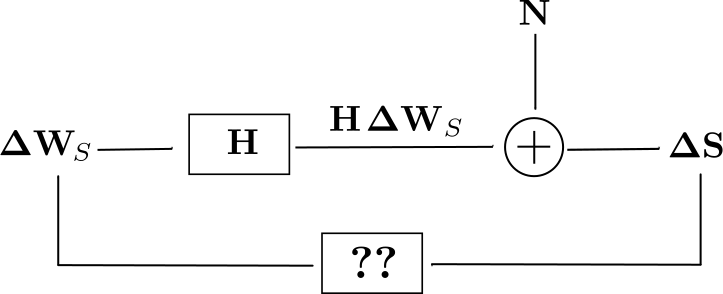
\includegraphics[width = 7cm]{./appA/direct_model}
	\caption{\textbf{Schematic representation of the direct model.} The measured excess noise is modelled as the convolution by a probe function plus some additional noise $N$. In this case we replace the convolution product by its equivalent matrix product $H$. The issue of this annex is to propose what can replace the question marks, and recover $\Delta W_{S}$ from $\Delta S$.}
	\label{fig: direct model}
\end{figure}

This schematic is the direct model and can be summarised in following equation \eqref{eq: direct model} :

\begin{equation}
\Delta S = H\Delta W_{\mathrm{S}}+N \label{eq: direct model}
\end{equation}

The problem is how to find $\Delta W$ for the measurement of $\Delta S$, as depict by the question marks in figure Fig. \ref{fig: direct model}. In other words it is how to inverse the direct model equation \eqref{eq: direct model}.



\subsection{\texorpdfstring{Why do we need a deconvolution method?}{Why we need a deconvolution method?}}

To support the explanation in this annex we can take the example of a 2GHz sine excitation at a temperature of 60mK and carrying one elementary charge e or -e per half-period. And we can focus on the deconvolution of its spectroscopy (or 0$^{\mathrm{th}}$ harmonic) measurement and the results on the whole Wigner function. To estimate the accuracy of different methods, we can compare the data get from measurements with ones get from theoretical calculations shown in figure Fig. \ref{fig: Theory}.

\begin{figure}[hptb]
	\begin{center}
		\begin{tabular}{c c}
			(a) &  \\ 
			
			& 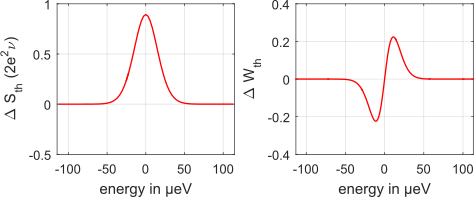
\includegraphics[width = 10 cm]{./appA/Th_result} \\
			
			(b) &  \\ 
			
			& 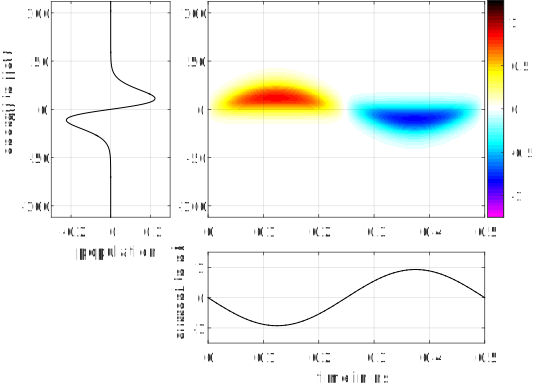
\includegraphics[width = 10 cm]{./appA/Th_wigner}
		\end{tabular} 
	\end{center}
	
	\caption{\textbf{Theoretical calculations on 2GHz sine example at a temperature of 60mK.} \textbf{(a)} left - Calculated theoretical noise $\Delta S_{\mathrm{th}}$ - right - Calculated theoretical spectroscopy $\Delta W_{\mathrm{th}}$. \textbf{(b)} The whole calculated theoretical Wigner function.}
	\label{fig: Theory}
\end{figure}


A naive approach is to discard the unknown noise and to just invert the known convolution matrix $H$, as represented in schematic (a) of figure Fig. \ref{fig: naive deconvolution}. If we look at the estimated result $H^{-1}\Delta S$ in figure Fig. \ref{fig: naive deconvolution} right graph of (b) panel, one can clearly remark that the estimator is dominated by only few oscillations. This result is clearly not reliable since these oscillations are several orders of magnitude stronger than expected result $\Delta W_{\mathrm{th}}$. This effect is not due a limited numerical precision in matrix inversion, because the re-convolution of the estimated solution $H\Delta W$ matches perfectly with the measured data $\Delta S$. The left graph of (b) panel in figure Fig. \ref{fig: naive deconvolution} shows this perfect agreement between $\Delta S$ and $H\Delta W$. Moreover the estimator is sensible to small error perturbations. In figure Fig. \ref{fig: naive deconvolution} panel (c), we add a small noise on measured data to get two very close data set $\Delta S$ and $\Delta S^{\prime}$. These two data set are barely discernible in left graph. But the two respectively estimated results $\Delta W$ and $\Delta W^{\prime}$ are very different. The last remark is that it also does not verify physical properties such as the Pauli exclusion principle for this spectroscopy measurement. The Pauli exclusion principle implies that the result $\Delta W$ plus the Fermi distribution $f_{\mathrm{fermi}}$ should be bounded between 0 and 1 as expressed by equation \eqref{eq: Pauli exclusion principle}:

\begin{equation}
	0 \leq \Delta W_{0}\left(E\right)+f_{\mathrm{fermi}}\left(E\right) \leq 1 \label{eq: Pauli exclusion principle} 
\end{equation}

And values on right graphs of figure Fig. \ref{fig: naive deconvolution} of the order of $10^{4}$ obviously violate the above inequality.

\begin{figure}[hptb]
	\begin{center}
\begin{tabular}{c c}
	(a) &  \\ 
	
	& 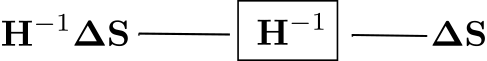
\includegraphics[width = 5cm]{./appA/naive_deconvolution} \\ 
	 
	(b) &  \\ 
	
	& 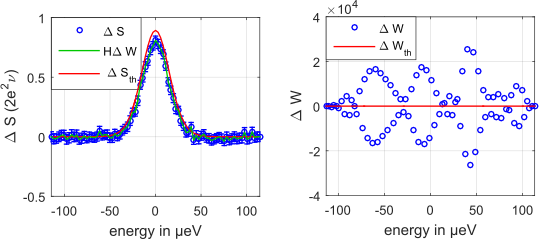
\includegraphics[width = 10 cm]{./appA/Naive_method_results} \\
	(c) &  \\ 
	
	& 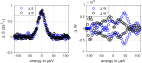
\includegraphics[width = 10 cm]{./appA/Naive_method_results_bis} 
\end{tabular} 
\end{center}
\caption{\textbf{Naive deconvolution method.} \textbf{(a)} Schematic of the naive inverse technique which just consists in multiplying experimental data by the inverse matrix $H^{-1}$. \textbf{(b)} left - Measured data $\Delta S$, calculated theoretical noise $\Delta S_{\mathrm{th}}$ and re-convoluted solution $H\Delta W$, all take similar values - right - Solution of the naive deconvolution $\Delta W$ which is order of magnitude greater than the theoretical solution $\Delta W_{\mathrm{th}}$. \textbf{(c)} left - Two measured data set $\Delta S$ and $\Delta S^{\prime}$ to which are added a random noise. These two data set take similar values. - right - Solution $\Delta W$ based on data points $\Delta S$, and solution $\Delta W^{\prime}$ based on data points $\Delta S^{\prime}$. These two solutions are very different even if the input data points are similar.}
\label{fig: naive deconvolution}
\end{figure}


This behaviour is explained by the fact that deconvolution is an ill-posed problem. This means that the $H$ matrix that model the convolution has some zero or close to zero eigenvalues. This can be shown in the Fourier space where the convolution is just the product by the Fourier transform of the convolution function $h$. And the Fourier transform components of $h$ posses some zeros or close to zero values. So inverting $H$ is equivalent to divide some Fourier component of $\Delta S$ per 0. Even if $H\Delta W$ vanishes for these components, the noise $N$ doesn't and the solution is completely dominated by these noise terms divided by 0.

\section{\texorpdfstring{The Fourier space technique: Wiener filter}{The Fourier space technique: Wiener filter}\label{sec: Wiener filter}}

%présenter technique wiener filtering

\subsection{\texorpdfstring{The optimal Wiener filter in ideal case}{The optimal Wiener filter in ideal case}}

The first technique to overcome the problem presented in above section \ref{sec: The deconvolution problem}, the Wiener filter \cite{wiener1949extrapolation}, is to filter the problematic Fourier components where the noise is divided by 0. The idea is to find the optimum filter that  gives the minimum distance between filtered result $FH^{-1}\Delta S$ and the original signal $\Delta W$. This distance has to be minimum for the average, denoted by $\left<.\right>$ over all different realization of the noise $N$ since it is unknown. This distance is given by \eqref{eq: Wiener criterion}.

\begin{equation}
	\left<\left|\left| FH^{-1}\Delta S - \Delta W \right|\right|_{2}^{2}\right> \label{eq: Wiener criterion}
\end{equation}

In Fourier space the filter $F$ and the matrix $H$ are diagonal, keeping the same symbols for thier diagonal part, we can find the optimum filter $F$ by solving the below equation \eqref{eq: Wiener developpement}.

\begin{equation}
	\frac{\mathrm{d}}{\mathrm{d}F}\left( \left<\left|\left| FH^{-1}\Delta S - \Delta W \right|\right|_{2}^{2}\right> \right) = 0 \label{eq: Wiener developpement}
\end{equation}

which gives the expression of the filter \eqref{eq: optimal Wiener filter}.

\begin{equation}
	F = \frac{HH^{\ast}}{HH^{\ast}+\left<\left|\frac{N}{\Delta W}\right|^{2}\right>} = \frac{1}{1+\left<\left|\frac{N}{H\Delta W}\right|^{2}\right>} \label{eq: optimal Wiener filter}
\end{equation}

This Wiener filter \cite{wiener1949extrapolation} is optimal because:
\begin{itemize}
	\item in the case of a convoluted signal higher than the noise $N\ll H\Delta W$ we get $\Delta S \sim H\Delta$. So we don't need to filter since $H^{-1}\Delta S \sim \Delta W$. This is indeed the case because in this limit $F \sim 1$.
	\item in the other case, the convoluted signal is smaller than the noise $H\Delta W\ll N$. This implies that we measure only noise $\Delta S \sim N$. The filter suppress this term since in this limit $F \sim \left<\left|\frac{H\Delta W}{N}\right|^{2}\right> \ll 1$.
\end{itemize}

\subsection{\texorpdfstring{The implemented Wiener filter}{The implemented Wiener filter}}

To construct this filter we need two quantities, first the noise spectrum $\left<\left|N\right|^{2}\right>$, which is measured if we assumed a white noise and thanks to repeated measurement. The second quantity is the spectrum of the solution $|\Delta W|^{2}$. But as it is the one we are looking for, we don't know it. So we need to use some hypothesis to approach the optimum filter. To do so the first one is that when $\Delta S \gg N$ we can assume $\Delta W \sim H^{-1}\Delta S$ and so the filter has the form \eqref{eq: Wiener filter use for high SNR}:

\begin{equation}
	F = \frac{1}{1+\left<\left|\frac{N}{\Delta S}\right|^{2}\right>} \label{eq: Wiener filter use for high SNR}
\end{equation}

When $\Delta S \sim N$ we know that $H\Delta W \leq N \sim \Delta S$ so we assumed that there is a corner point where $\Delta W \leq \Delta W(\tau_{c}) \sim \frac{\Delta S(\tau_{c})}{H(\tau_{c})}  \sim \frac{N}{H(\tau_{c})}$ and we use it as a boundary for our filter by replacing $H\Delta W$ by $\frac{HN}{H(\tau_{c})}$ like in \eqref{eq: Wiener filter use for low SNR}:

\begin{equation}
	F = \frac{1}{1+\left|\frac{H(\tau_{c})}{H}\right|^{2}} \label{eq: Wiener filter use for low SNR}
\end{equation}

We end up with the following filter \eqref{eq: Wiener filter used}

\begin{eqnarray}
	F &=& \frac{1}{1+\left<\left|\frac{N}{\Delta S}\right|^{2}\right>}\; \mathrm{when}\; H \geq H(\tau_{c}) \\
	&=& \frac{1}{1+\left|\frac{H(\tau_{c})}{H}\right|^{2}}\; \mathrm{when}\; H \leq H(\tau_{c}) \\ \label{eq: Wiener filter used}
\end{eqnarray}

The implementation of this filter in the deconvolution process sketched in the figure Fig. \ref{fig: Wiener_results} panel (a), gives the results of the two lower panels (b) and (c). On right graph of panel (b), the estimated solution $\Delta W$ is comparable with the computed one $\Delta W_{\mathrm{th}}$. On the left graph of panel (b) the re-convoluted estimator $H\Delta W$ still matches the measured data $\Delta S$, even if we filter the deconvolved estimator. It shows that by filtering we do not alter the information given by our measurements. Some points of $\Delta S$ in the middle of the central peak are distant from the computed $\Delta S_{\mathrm{th}}$, and this might explain why at the peaks location some points of $\Delta W$ are also distant from $\Delta W_{\mathrm{th}}$. An effect which is well reproduced by measured points $\Delta S$, is that at high energies, $\left|E\right|\geq 50 \mu$eV, $\Delta S_{\mathrm{th}}$ is flat at zero value. But the estimator $\Delta W$ or the re-convoluted estimator $H\Delta W$ do not capture this effect and display some small unexpected oscillations at these energies. These oscillations induced some unwanted yellow and cyan spots in the total Wigner function of panel (c) and the current shows some deviations from a sine function.

To compute error bars on the estimators $\Delta W$, we assume a white noise whose power is given by repeated measurement $V_{e}=\left<\Delta S^{2}\right>-\left<\Delta S\right>^{2}$. Than error bars are given by $\sigma = \sqrt{f_{\mathrm{sampling}}\int\limits_{0}^{+\infty}\mathrm{d}\tau \left|\frac{F\left(\tau\right)}{H\left(\tau\right)}\right|^{2}V_{e}}$

\begin{figure}[hptb]
		\begin{center}
		\begin{tabular}{c c}
			(a) &  \\ 
			
			& 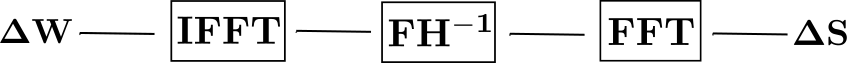
\includegraphics[width = 8 cm]{./appA/Wiener_deconvolution} \\ 
			
			(b) &  \\ 
			
			& 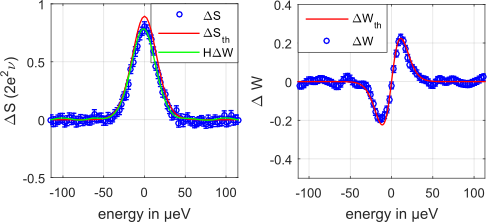
\includegraphics[width = 10 cm]{./appA/Wiener_results} \\
			
			(c) &  \\ 
			
			& 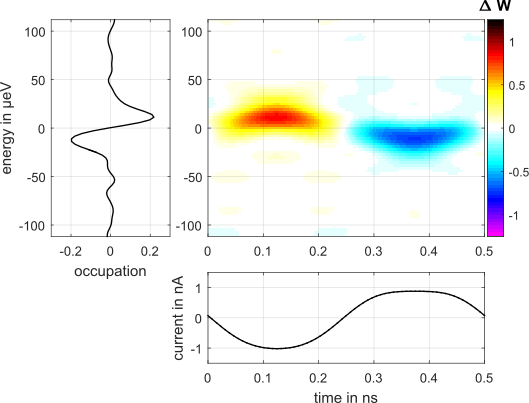
\includegraphics[width = 10 cm]{./appA/Wiener_result_wigner}
		\end{tabular} 
	\end{center}
	\caption{\textbf{Wiener deconvolution filter.} \textbf{(a)} Schematic of Wiener deconvolution technique, the inversion $H^{-1}$ and the filtering $F$ are performed in Fourier space since it is then reduced to a simple product. Indeed in the Fourier basis $H$ is diagonal. \textbf{(b)} left - Measured data $\Delta S$, calculated theoretical noise $\Delta S_{\mathrm{th}}$ and re-convoluted solution $H\Delta W$, all take similar values - right - Solution of the Wiener deconvolution $\Delta W$ which is consistent with expected calculations $\Delta W_{\mathrm{th}}$, except for some oscillations at high energies. \textbf{(c)} The whole Wigner function deduced from measurements thanks to Wiener deconvolution.}
	\label{fig: Wiener_results}
\end{figure}

\section{\texorpdfstring{The Bayesian framework}{The Bayesian framework}}

The Wiener filter in the above section \ref{sec: Wiener filter} gives a reasonable solution compared to the issue raise in figure Fig. \ref{fig: naive deconvolution}. And it has been successfully used for studying electron tomography in \cite{marguerite2017extracting} and \cite{marguerite2017two}. But it can still be improved like for example on the high energy oscillations.

The Wiener technique limitation is as we don't know the power spectrum of the solution, we are forced to use hypothesis that don't correspond to physical properties. To get a solution which verify known physical properties, we introduce a new problem formulation, the Bayesian framework \cite{ayasso2010joint}, \cite{mohammad2015bayesian}, \cite{zhao2016joint}.  The measurement is the mean, or equivalently the maximum, of the probability distribution of $\Delta S$ knowing the searched quantity $\Delta W$ and the variance $V_{e}$ of Gaussian noise $N$. This probability distribution \eqref{eq: likelyhood} is called the likelihood. 

\begin{equation}
	p\left(\Delta S | \Delta W, V_{e} \right) \propto \exp\left(-\frac{1}{2}||\Delta S - H\Delta W||_{V_{e}}^{2}\right)\;\mathrm{with}\;||x||_{V_{e}}^{2} = \sum_{i}^{}\frac{|x_{i}|^{2}}{V_{e,i}} \label{eq: likelyhood}
\end{equation}

But what we are looking for is $\Delta W$. So we are interested in the probability distribution of $\Delta W$ knowing the measurement $\Delta S$ and the noise variance $V_{e}$. Thanks to Bayes'formula \eqref{eq: Bayes'formula} we can link these two probability distributions.

\begin{equation}
	p\left(\Delta W |\Delta S , V_{e} \right)p\left(\Delta S\right) = p\left(\Delta S | \Delta W, V_{e} \right)p\left(\Delta W \right) \label{eq: Bayes'formula}
\end{equation}

We can expressed the probability distribution of interest $p\left(\Delta W |\Delta S , V_{e} \right)$, thanks to the measurement with likelihood $p\left(\Delta S | \Delta W, V_{e} \right)$ and to a prior knowledge on the solution with $p\left(\Delta W \right)$. The a priori informations encoded in the so-called prior distribution function $p\left(\Delta W \right)$ is a much more convenient way to enforce physical properties. For example we choose a Gaussian prior
distribution \eqref{eq: prior distribution annexe} on $\Delta W$

\begin{equation}
p\left( \Delta W \right)  \propto  
\exp\left(
-\frac{1}{2}\left\| \Delta W \right\|^{2}_{V_{f}}  
\right).
\label{eq: prior distribution annexe}
\end{equation}
For variances $V_{f}$, we use the expression \eqref{eq:variances Vf} where $v_f$ and $w$ are parameters tuned to enforce limit condition when energy $\left|E \right|$ increases. This limit condition corresponds to the physical properties that there is less signal at high energy than at low energy.

\begin{equation}
V_{f}\left(E\right) = v_{f}\exp \left( -\frac{E^{2}}{w^{2}} \right)
\label{eq:variances Vf}
\end{equation}

\subsection{\texorpdfstring{Posterior law maximization}{Posterior law maximization}\label{sec: MAP}}

%présenter le framework Bayesian avec MAP

%un peu dire que ce qu'on cherche c'est le max de la loi de probabilité. qu'on peut dire comme a priori qu'on cherche le signal de norme 2 minimum et qu'on préviligie les petites énergies aux grandes. et donc on a juste besoin de trouver le minimum de -log(p) soit du critère J. et que ça on peut le donner analytiquement par ...

In this framework we can define our solution as the most likely $\Delta W$ knowing our measurement points $\Delta S$, their variances $V_{e}$, and the a priori information $V_{f}$. This is the argument which maximise the posterior probability distribution $p\left(\Delta W |\Delta S , V_{e} \right)$. It is equivalent to look for the minimum of the criteria \eqref{eq: MAP criterion}.

\begin{equation}
J\left(\Delta W\right) = - \ln\left(p\left(\Delta W |\Delta S , V_{e} \right)\right) = \frac{1}{2}||\Delta S - H\Delta W||_{V_{e}}^{2}+\frac{1}{2}||\Delta W||_{V_{f}}^{2} \label{eq: MAP criterion}
\end{equation}

Its minimum found by solving $\frac{\mathrm{d}J\left(\Delta W\right)}{\mathrm{d}\Delta W}  = 0$ is the analytical expression \eqref{eq: MAP equation} called maximum a posteriori \cite{fessler1996mean}, \cite{pereyra2017maximum}.

\begin{equation}
\Delta W = F\Delta S = \left(H^{\top}V^{-1}_{e}H+V^{-1}_{f}\right)^{-1}H^{\top}V^{-1}_{e}\Delta S \label{eq: MAP equation}
\end{equation}

On figure Fig. \ref{fig: MAP deconvolution} are plotted the results given by the maximum a posteriori. On the result plotted in the right graph of panel (b) we can noticed that the oscillations at energies $\left|E\right| \geq 50 \mu$eV are suppressed. And also on the Wigner function of panel (c) spots in the same energy range are removed. This effect induced by added a priori information, does not alter the solution found for low energies $\left|E\right| \leq 50 \mu$eV. In addition it also improve in the low energy range the expected electron-hole symmetry. We can remark on panel (b) that the re-convoluted solution $H\Delta W$ looks more symmetric between positive and negative energies. And that the current deduced from the Wigner function in panel (c) is closer to a sine function.

\begin{figure}[hptb]
	\begin{center}
		\begin{tabular}{c c}
			(a) &  \\ 
			
			& \includegraphics[width = 4 cm]{./appA/MAP_deconvolution} \\ 
			
			(b) &  \\ 
			
			& 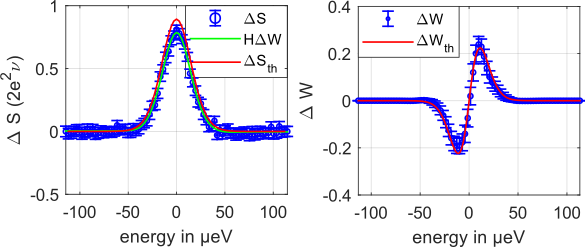
\includegraphics[width = 10 cm]{./appA/MAP_results} \\
			
			(c) &  \\ 
			
			& 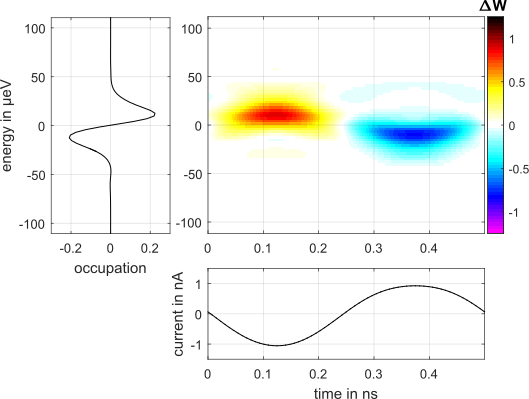
\includegraphics[width = 10 cm]{./appA/MAP_wigner}
		\end{tabular} 
	\end{center}
	
	\caption{\textbf{Maximum A Posteriori deconvolution.} \textbf{(a)} Schematic of MAP deconvolution, the inversion is performed by one matrix product $F$ in the direct space. Some a priori information $V_{f}$ is added to compute the matrix $F$. \textbf{(b)} left - Measured data $\Delta S$, calculated theoretical noise $\Delta S_{\mathrm{th}}$ and re-convoluted solution $H\Delta W$. - right - Solution of the MAP deconvolution $\Delta W$, as expected from $\Delta W_{th}$ the high energy oscillations are suppressed. \textbf{(c)} The whole Wigner function deduced from measurements thanks to MAP. Yellow and blue spots at energies above 50 $\mu$eV are removed.}
	\label{fig: MAP deconvolution}
\end{figure}


We choose as solution the maximum of the posterior distribution to get an analytical formula, but it also corresponds in this case to the mean of the posterior distribution \cite{bardsley2012mcmc} \cite{howard2014sampling}. The panel (a) of figure Fig. \ref{fig: PM_for_MAP} display the solution estimated from the posterior mean, and we can check that it corresponds to the maximum a posteriori. To deduce the posterior mean, we compute the posterior probability distribution, thanks to random draws following the product of likelihood and prior distribution. In panel (b) we plotted for energy point $E$ the histogram of $\Delta W\left(E\right)$ values found. These histograms give a representation of the solution of posterior distribution. We can remark on these histograms that a priori information allows the posterior distribution to be more spread for low energy values $|E|\leq 50 \mu$eV than for higher ones.

\begin{figure}[hptb]
	\begin{center}
		\begin{tabular}{c c}
			(a) &  \\ 
			
			& 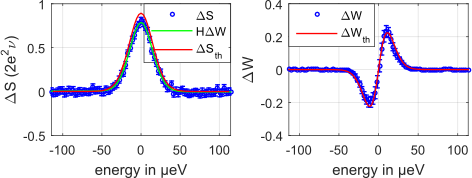
\includegraphics[width = 10 cm]{./appA/PM_for_MAP_posterior_distribution} \\ 
			
			(b) &  \\ 
			
			& 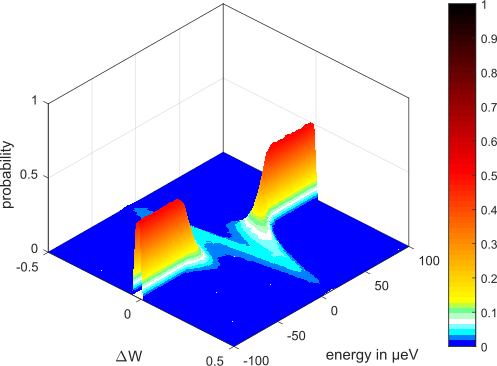
\includegraphics[width = 10 cm]{./appA/MAP_posterior_distribution}
		\end{tabular} 
	\end{center}
	
	\caption{\textbf{Random draws following the posterior distribution.} \textbf{(a)} Solution deduce from the mean of random draws on the posterior distribution. We found the same result as for the maximum a posteriori. \textbf{(b)} Each line along the x-axis is an histogram of solution $\Delta W\left(E\right)$ values for one energy $E$. Values on the z-axis are computed from the percentage of value $\Delta W\left(E\right)$ among the random draws.}
	\label{fig: PM_for_MAP}
\end{figure}


But it does not directly give the error bars plotted on solution $\Delta W$. The error bars correspond to the standard deviation of the deduce $\Delta W$ estimated over different input data $\Delta S$ set with different realization of measurement noise $N$. Whereas the posterior distribution spread is due both to the noise $N$ in the likelihood but also to the prior distribution. Rather than posterior distribution width, the error bars correspond to the fluctuation of its maximum when we add a noise $N$ to the input data set $\Delta S$. To compute these error bars, we performed an analytical calculation of  the covariance matrix $\Sigma_{\Delta W}$ of $\Delta W$ \eqref{eq: MAP covariance} thanks to the analytical expression \eqref{eq: MAP equation}, \cite{fessler1996mean}.

\begin{equation}
\Sigma_{\Delta W} = \left<\Delta W^{2}\right>-\left<\Delta W\right>^{2} = \left(H^{\top}V^{-1}_{e}H+V^{-1}_{f}\right)^{-1}H^{\top}V^{-1}_{e}H\left(H^{\top}V^{-1}_{e}H+V^{-1}_{f}\right)^{-1} \label{eq: MAP covariance}
\end{equation}

This covariance matrix $\Sigma_{\Delta W}$ is plotted on the right of figure Fig. \ref{fig: MAP_covariance}. It is consistent with the covariance matrix plotted on its left, which is computed thanks to random draws of measurement points $\Delta S$ plus a realization of noise $N$. We use only the analytic covariance matrix diagonal part to plot error bars on graphs. But to compute the error bars of extracted quantity from the whole Wigner function such as populations, we use the full covariance matrix.

\begin{figure}[hptb]
	\begin{center}		
	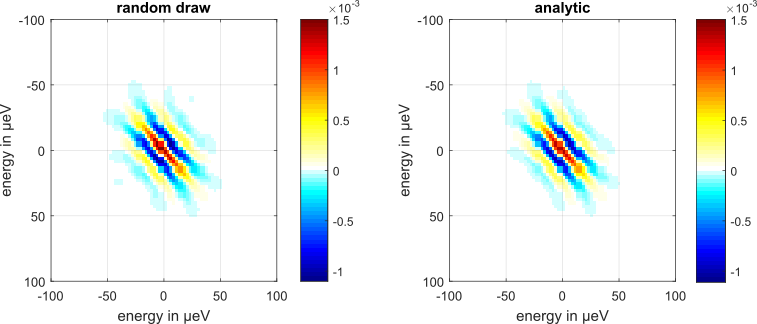
\includegraphics[width = 12 cm]{./appA/MAP_covariance}
	\end{center}
	\caption{\textbf{Covariance matrix of Maximum a posteriori solution.} left - covariance matrix estimated for random draws of input data $\Delta S$ plus a drawn noise $N$ - right - covariance matrix estimated by analytical calculation. These two methods show the same results.}
	\label{fig: MAP_covariance}
\end{figure}


%aidez la présentation avec le direct sampling

%dire qu'on peut faire un tirage au sort pour avoir l'histogramme de valeurs qui suit la loi de la distribution a posteriori et montrer que ça donne le même résultat

%dire qu'on peut aussi donner des barres d'erreur en calculant tout simplement ... mais que attention c'est pas la même chose que la largeur de loi a posteriori, c'est la variation du maximum de la loi a posteriori.

\subsection{\texorpdfstring{Unsupervised technique with joint posterior law maximization}{Unsupervised technique with joint posterior law  maximization}\label{sec: JMAP}}

%présenter le un-supervised avec JMAP

In the above method we impose the values of $V_{f}$, but we don't know their values, so we can replace it by an inverse-gamma probability distribution  law \eqref{eq: hyper-priors inverse gamma law} of shape parameter $\alpha$ and scale $\beta$.

\begin{equation}
p\left(V_{f}|\alpha, \beta \right) \propto \left(\frac{1}{V_{f}}\right)^{\alpha+1}\times\exp\left(-\frac{-\beta}{V_{f}}\right) \label{eq: hyper-priors inverse gamma law}
\end{equation}

What we are now searching is the most likely values of $\Delta W$ and $V_{f}$ knowing measurements points $\Delta S$, their variances $V_{e}$, and parameters $\alpha$, $\beta$. So the posterior law \eqref{eq: JMAP posterior law} is re-expressed due to Bayes'rule.

\begin{equation}
p\left(\Delta W, V_{f} |\Delta S , V_{e}, \alpha, \beta \right) \propto p\left(\Delta S | \Delta W, V_{e} \right)p\left(\Delta W | V_{f} \right)p\left(V_{f} | \alpha, \beta\right) \label{eq: JMAP posterior law}
\end{equation}

To converge towards both $\Delta W$ and $V_{f}$ which maximise the posterior, we performed an alternate optimization of $p\left(\Delta W |\Delta S , V_{e}, V_{f} \right)$ and $p\left(V_{f} |\Delta S , V_{e},\Delta W  \right)$ \cite{mohammad2015bayesian}, \cite{ayasso2010joint}, \cite{zhao2016joint}. This joint maximization is performed by alternatively updating the value of $\Delta W$ as previously thanks to formula \eqref{eq: MAP equation}, than updating the value of $V_{f}$ thanks to formula \eqref{eq: Vf updates formula}.

\begin{equation}
V_{f} = \frac{\beta+\frac{1}{2}\Delta W^{2}}{\alpha+\frac{3}{2}} \label{eq: Vf updates formula}
\end{equation}

For this new method, formula \eqref{eq: prior distribution} is only used to initialize $V_{f}$ and $\beta = \left(\alpha+1\right)V_{f}$. The value of $\alpha$ determines the closeness of the optimized $V_{f}$ to initialization \eqref{eq: prior distribution}.

On figure Fig. \ref{fig: JMAP deconvolution}, we remark that in this JMAP case there are almost no difference with above MAP technique section \ref{sec: MAP}.

\begin{figure}[hptb]
	\begin{center}
		\begin{tabular}{c c}
			(a) &  \\ 
			
			& \includegraphics[width = 4 cm]{./appA/JMAP_deconvolution} \\ 
			
			(b) &  \\ 
			
			& 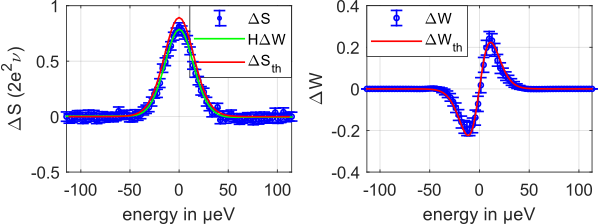
\includegraphics[width = 10 cm]{./appA/JMAP_result} \\
			
			(c) &  \\ 
			
			& 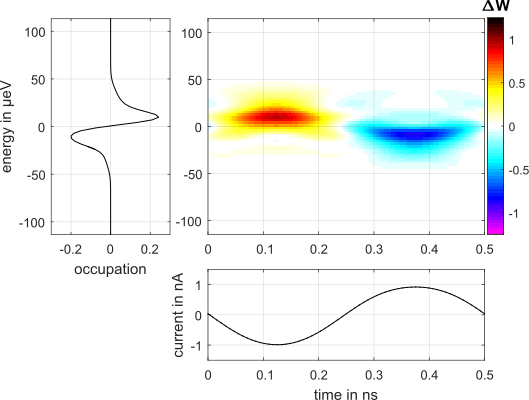
\includegraphics[width = 10 cm]{./appA/JMAP_wigner}
		\end{tabular} 
	\end{center}
	
	\caption{\textbf{Joint Maximum A Posteriori deconvolution.} \textbf{(a)} Schematic of JMAP deconvolution, the inversion is performed by one matrix product $F$ in the direct space. The solution is used to optimize the values of $V_{f}$ parameters, which follow an Inverse-Gamma law of shape parameter $\alpha$ and scale parameter $\beta$. After several loop step between $F$ and $V_{f}$ we get the solution $F\Delta S$. \textbf{(b)} left - Measured data $\Delta S$, calculated theoretical noise $\Delta S_{\mathrm{th}}$ and re-convoluted solution $H\Delta W$. - right - Solution of the JMAP deconvolution $\Delta W$, which is similar to the solution given by the MAP method. \textbf{(c)} The whole Wigner function deduced from measurements thanks to JMAP.}
	\label{fig: JMAP deconvolution}
\end{figure}


%The schematics of this algorithm is show on figure \ref{fig: JMAP deconvolution}. This gives the results show in figure \ref{fig: JMAP deconvolution}.

%aidez la présentation avec la Monte-Carlo-Markov-Chain ou pas

\subsection{\texorpdfstring{Box constrained problem with projected gradiant}{Box-constraint problem with projected gradiant}}

%présenter la box-constraint et le gradient projeté

The above technique allows to add some a priori information like a high energy cut-off. But still some physical properties are missing. The ones added in this section is the Pauli exclusion principle and the Cauchy-Schwartz inequality \cite{ferraro2013wigner}. The Pauli exclusion principle enforces that the result of the 0$^{\mathrm{th}}$ harmonic of the Wigner function (or spectroscopy) plus the Fermi distribution has to be bounded between 0 and 1, see equation \eqref{eq: Pauli exclusion principle}. This inequality condition define a box in which the solution has to be found. This kind of problem is common in image processing, where grey pixel values are bounded between 0 and 255, it is called a box-constrained problem \cite{afonso2011augmented} \cite{lanteri2002penalized} \cite{chan2012multiplicative} \cite{bardsley2012mcmc2}. To look for a solution inside the box defined by the Pauli exclusion principle, we perform a projected gradient descent method \cite{figueiredo2007gradient} \cite{bertsekas1997nonlinear}.

This method follows the drawing of figure Fig. \ref{fig: ProjGrad descent}. First we initialize the solution by projecting the maximum a posteriori solution $\Delta W_{\mathrm{MAP}}$ given by equation \eqref{eq: MAP equation} inside the box by \eqref{eq: solution projection inside box}.

\begin{eqnarray}
\Delta W_{\mathrm{init}} = \min\left(\max\left(\Delta W_{\mathrm{MAP}} ,-\mathrm{fermi} \right),1-\mathrm{fermi} \right)  \label{eq: solution projection inside box}
\end{eqnarray}

The criterion $J\left(\Delta W\right)$ \eqref{eq: MAP criterion} gives the value we have to minimize. So we can compute its gradient $\nabla J\left(\Delta W\right)$ \eqref{eq: gradient} at the previous value of $\Delta W_{\mathrm{init}}$.

\begin{equation}
\nabla J\left(\Delta W_{\mathrm{init}}\right) = -H^{\top}V^{-1}_{e}\left(\Delta S-H\Delta W_{\mathrm{init}}\right)+V^{-1}_{f}\Delta W_{\mathrm{init}} \label{eq: gradient}
\end{equation}

And project it to stay in the box by setting at zero all components that point outside of the box when $\Delta W_{\mathrm{init}}$ is at a boundary of the box. We can also compute the optimum displacement along direction given by the gradient computed in \eqref{eq: gradient}, and performed one descent step to find $\Delta W_{\mathrm{Proj.Grad.}}$. Than as in the previous section \ref{sec: JMAP} we performed an alternate optimization by updating the values of $V_{f}$ thanks to formula \eqref{eq: Vf updates formula}. To perform the whole descent we return to the gradient calculation step to perform several iteration until the joint posterior law is maximized under the box constraints imposed by Pauli exclusion principle. For harmonics one to five, the box boundary are given by the solution of the zero harmonic thanks to Cauchy-Schwartz inequality.

This algorithm gives the result in figure Fig. \ref{fig: ProjGrad deconvolution}. Almost all the un-expected cyan and yellow spots included at low energies have been suppressed, compare to the Wiener filtering result in figure Fig. \ref{fig: Wiener_results}.


\begin{figure}[hptb]
	\centering
	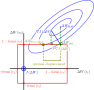
\includegraphics[width = 10 cm]{./appA/gradient_descent_schematics}
	\caption{\textbf{Projected gradient descent schematic.} In red the box given by the Pauli exclusion principle. In blue the criterion given by the posterior distribution law. In green projection for the initial value and the gradient. In gold solution given by the algorithm, which is the lowest value of the criterion in the box given by the Pauli exclusion principle.}
	\label{fig: ProjGrad descent}
\end{figure}

\begin{figure}[hptb]
	\begin{center}
		\begin{tabular}{c c}
			(a) &  \\ 
			
			& \includegraphics[width = 8 cm]{./appA/ProjGrad_deconvolution} \\ 
			
			(b) &  \\ 
			
			& 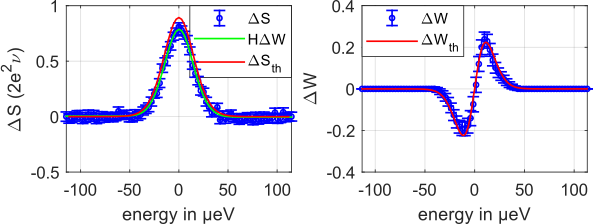
\includegraphics[width = 10 cm]{./appA/PG_result} \\
			
			(c) &  \\ 
			
			& 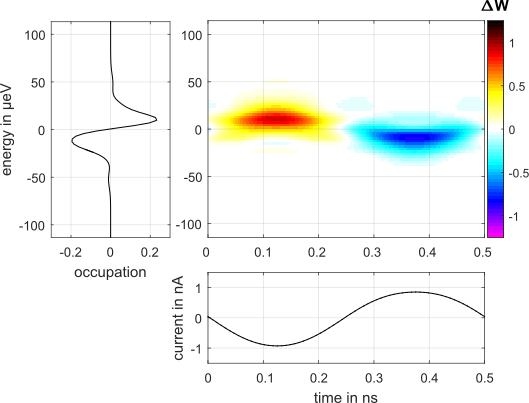
\includegraphics[width = 10 cm]{./appA/PG_wigner}
		\end{tabular} 
	\end{center}
	
	\caption{\textbf{Projected Gradient deconvolution method.} \textbf{(a)} Schematic of the deconvolution method, first a MAP deconvolution is performed. Its solution $F\Delta S$ is projected by $P$ in the box $M$. Than starting from this initial value, one projected gradient descent step and one update of $V_{f}$ values are repeated at each loop step \textbf{(b)} left - Measured data $\Delta S$, calculated theoretical noise $\Delta S_{\mathrm{th}}$ and re-convoluted solution $H\Delta W$. - right - Solution of the deconvolution $\Delta W$. \textbf{(c)} The whole Wigner function deduced from measurements. Almost all unexpected yellow and cyan spots are erased even in the energy range below 50 $\mu$eV.}
	\label{fig: ProjGrad deconvolution}
\end{figure}

\section{\texorpdfstring{Outlook: toward a 2D treatment}{Outlook: toward a 2D treatment}}

%mettre en perspective le full traitement 2D

The Wiener filtering method have already been investigated in the PhD\cite{marguerite2017two}, in this section we develop and demonstrate a more robust method which enable to enforce physical properties on the solution. This improve the deconvolution results especially for signal going to higher energies. But still some improvements can be made. The above method is succession of 1D deconvolution, where we use the first one to impose the Cauchy-Schwartz inequality to all others harmonics as sketch in figure Fig. \ref{fig: 1D->2D deconvolution} panel (a). This is an improvement toward the use of all harmonics, but it is not yet a full 2D deconvolution, where the presence of signal in higher harmonics could suggest that there are some signal at the harmonic 0$^{\mathrm{th}}$. So an improved version could be to deconvolve simultaneously all harmonics as depict in figure Fig. \ref{fig: 1D->2D deconvolution} panel (b).

\begin{figure}[hptb]
	\begin{center}
		\begin{tabular}{c c c c}
			(a) & & (b) &  \\ 
			
			& \includegraphics[scale = 0.25]{./appA/1D_deconvolution} & & 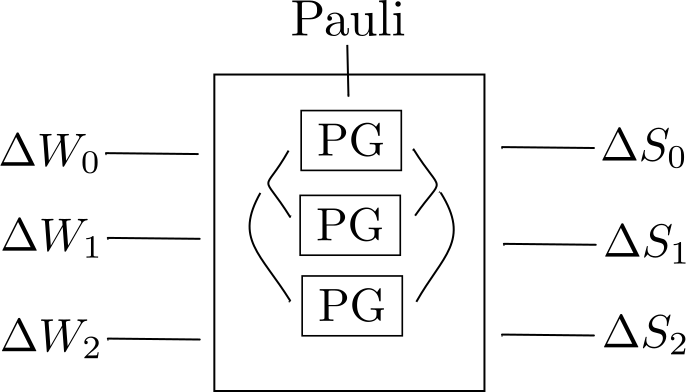
\includegraphics[scale = 0.25]{./appA/2D_deconvolution} 
		\end{tabular} 
	\end{center}

	\caption{\textbf{From 1D to 2D deconvolution.} \textbf{(a)} - succession of 1D Project Gradient deconvolution method used in this manuscript - \textbf{(b)} - perspective of a 2D deconvolution method.}
	\label{fig: 1D->2D deconvolution}

\end{figure}

